% sections/interp_dyn.tex: part 2 of \cref{sec:interp} ("What it learns"), \input at the end of sections/interp.tex:
% the two regimes, the failures, false admissions and the order of acquisition.  Figures and tables come from
% make_interp.py; the numbers quoted here that no figure or table shows are stored in tables/interp_numbers.json, or
% come from the analysis reports and their outputs that the text names (THEORY.md, ORDER.md, CALIB.md, ABLATIONS.md).
% The full versions of these subsections are in sections/app_interp.tex.

% ======================================================================================================================
\subsection{Two regimes: when the structure appears, and when its test would admit it}\label{sec:interp-when}

Apart from the forced variant's guesses, each piece of a target's structure has two sizes: the training-set size from which DFG's test would admit it if the search offered it, and the size from which the model holds it. For characters the search offers every candidate of a class; for sum blocks it offers only blocks grown from statistics of one or two inputs (\cref{prop:blocks}), so the two sizes can be far apart. This subsection measures both and then moves the tests' threshold (detail in \cref{app:interp-when}).

\begin{figure}[tbp]
\centering
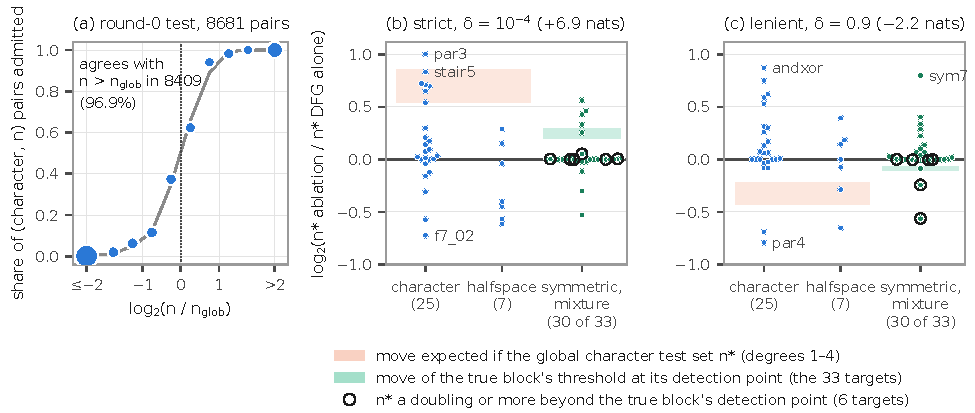
\includegraphics[width=\linewidth]{figures/fig_dyn_when.pdf}
\caption{The test and the data cost. (a)~DFG's round-0 decisions on the target characters of degree $\le4$ against the detection size $n_{\rm glob}$ (41 \code{designed} and \code{random} targets, seed 0, every grid size; 8681 (character, $n$) pairs) \status{Numerical}: the share admitted in each band of $\log_2(n/n_{\rm glob})$ (area $\propto\sqrt{\text{pairs}}$; end bands open), and a normal approximation for $v_S$ (line). (b, c)~\code{strict} and \code{lenient}: $\log_2(\nstar_{\rm ablation}/\nstar_{\rm DFG\ alone})$ per target (seeds 0 and 1, paired), by the ablation analysis's class; the three residue classes, which neither run learns, are not drawn \status{Numerical}. Orange: the move of $n_{\rm glob}$ for one character of degree 1--4, the move of $\nstar$ if a round-0 character test set it \status{Heuristic}. Green: the range of the true block's threshold move at its detection point over the 33 symmetric and mixture targets \status{Numerical}. Rings: the 6 targets whose $\nstar$ lies a doubling or more beyond that point (\cref{app:interp-when}). Sources: \repo{study/part11/interp/theory/check_theory.json} (\texttt{P3.test0}), \repo{study/part11/RESULTS.json} (\texttt{q5\_ablations}), \repo{study/part11/interp/ablations/ablations.json} and \repo{study/part10/interp/tables/toy_timing.csv}, via \repo{paper_dfg/make_interp.py}.}
\label{fig:dyn-when}
\end{figure}

\paragraph{Characters: admitted by detectability} \status{Proved, then Numerical}. In round 0 a character $\chi_S$ of degree $k$ searched on all rows passes its test exactly when $n>2c^2L_k\,s^2/v_S^2$ (\cref{prop:nglob}); replacing $v_S$ by the target's coefficient $\hat f(S)$ and $s^2$ by $1-\hat f(\emptyset)^2$ gives the \emph{detection size} $n_{\rm glob}(S)$ of \cref{eq:nglob}, a first-order prediction \status{Heuristic}. Degree enters only through the logarithm: with $K=4$, $\delta=0.1$ and $c=1$, $L_k$ is 8.5, 11.2, 13.4 and 15.3 nats for $k=1$--4 at $d=30$, so a coefficient $\sqrt{15.3/8.5}=1.34$ times larger at degree 4 than at degree 1 already has the smaller $n_{\rm glob}$. On the 41 targets of \code{designed} and \code{random}, DFG's round-0 decision agrees with ``admit when $n>n_{\rm glob}$'' in 8409 of 8681 (character, $n$) pairs (96.9\%; \cref{fig:dyn-when}a), and the 249 characters that first enter through this test do so at a median $2^{0.26}\,n_{\rm glob}$. The classes of later rounds admit characters a median 1.4 to 3.7 doublings below $n_{\rm glob}$, mainly because the residual there is 3.2 to 19 times smaller (class medians; \cref{tab:dyn-when}a): once the large terms are fitted, characters on the inputs already in use pass the tests of small classes, which resembles the junta completion that Part~5 saw in the networks \cite{gdcircuit2026} \status{Heuristic}. For a parity no search stands between the test and the model: \cref{prop:parity}'s criterion holds in all 250 parity cells with $n\ge32$.

\paragraph{Sum blocks: detection is cheap, discovery lags} \status{Numerical}. Part~10 measured both sizes for v3's DFG member on the 54 sum-structured targets \cite{portfoliolearner2026}: $n_{\rm detect}$, the first grid size at which DFG's block test would admit the target's \emph{true} block if it were proposed in round 0 (an oracle), and $n_{\rm struct}$, the first at which the model holds every signed-symmetry class of size $\ge3$ exactly. Over the 49 found, with the detection points that Part 10's verifier corrected for the gate and multiplexer mixtures, $n_{\rm struct}$ is earlier than $n_{\rm detect}$ for 6, equal for 20, one doubling later for 9 and two or more doublings later for 14, and the delay grows as the target's share of variance at Fourier degrees 1--2 shrinks (Spearman $-0.54$ over all 54). Part 10 labelled its reading, that the search sets the data cost, Heuristic: nothing isolated the search, and the stacker's choice between DFG's two variants could also have contributed. On the 13 sum-structured targets of the atlas DFG alone's $n_{\rm struct}$ equals that of v3's member (\cref{tab:dyn-when}b): the delay is 0 for 4, one doubling for 3, and two to six doublings for f7\_08, band11 and h5s7, and three never reach it. When the block enters, its statistic is well above the threshold (in Part~10's runs, a median 2.3 times at $n_{\rm struct}$ over the 22 pure symmetric targets found, range 0.89--74).

\paragraph{Moving the threshold} \status{Numerical, then Heuristic}. \code{strict} ($\delta=10^{-4}$) adds 6.9 nats to the log term of every test, and \code{lenient} ($\delta=0.9$) subtracts 2.2 (\cref{sec:ablations}; \repo{study/part11/interp/ablations/ABLATIONS.md}, post hoc, corrected after an independent verification). If a round-0 character test set $\nstar$, \code{strict} would raise it by $+0.54$ (degree 4) to $+0.86$ doublings (degree 1) \status{Heuristic}. The block test's log term is larger (33.7 nats for an unmodulated 11-input block), so at the true blocks' detection points \code{strict} moves its threshold by only $+0.20$ to $+0.30$ doublings of $n$ (re-thresholded post hoc; approximate for the modulated blocks, whose statistic was stored only as a ratio to its threshold). \Cref{fig:dyn-when}b,c shows what happened.
\begin{itemize}
\item \emph{Parities: the test sets the cost exactly.} \Cref{prop:parity} with $\delta$ moved, applied to each training set's own $\bar y$, predicts the measured changes to within 0.03 (par3 $+0.98$ against $+1.00$ under \code{strict}; par4 $-0.79$ against $-0.79$ under \code{lenient}).
\item \emph{Other character targets: one grid step where the test binds.} \code{strict} raises $\nstar$ by more than 0.25 on 8 of the 25, mostly by about the predicted amount. \code{lenient} is not the mirror image (2 lower, 8 higher): those targets are first fitted at small $n$, mostly by the forced variant, and with $\delta=0.9$ the linear block enters and the cross-validation's choice of variant changes (\cref{sec:abl-test}).
\item \emph{Halfspaces: a stricter test helps} ($-0.23$; $-0.17$ counting f7\_10): a degree-1 character that passes first takes part of the block's signal (\cref{app:interp-when}).
\item \emph{Symmetric and mixture targets: $\nstar$ stays} (class means $+0.04$ and $+0.05$; 30 of the 33 learned). On the 6 targets whose $\nstar$ lies a doubling or more beyond $n_{\rm detect}$ (band11, f7\_08, h6\_01, h6\_02, h6\_06, h6\_08; ringed in \cref{fig:dyn-when}), \code{strict} changes $\nstar$ by at most 0.05, although it moves their blocks' threshold by about a quarter of a doubling. These use the corrected detection points; with the uncorrected points, which the ablation analysis uses, there are 7 (f7\_03 as well, on which \code{strict} changes $\nstar$ by 0.00). On the other 24, $\nstar$ lies less than a doubling beyond $n_{\rm detect}$, and for 20 of them at or below it (23 and 18 with the uncorrected points), so the grid cannot separate the test from the search.
\end{itemize}
\emph{Reading} \status{Heuristic}. Where $\nstar$ lies a doubling or more beyond $n_{\rm detect}$, a test about a quarter of a doubling stricter changes nothing, because once the search proposes the block, the test admits it well above its threshold: \emph{there the search, not the test, sets the data cost}; on the other sum targets the grid cannot tell the two apart. Where the first fit comes from a character test, the test binds and $\nstar$ moves with the threshold: exactly for the parities, within a grid step for the staircases and small formulas. Where the first fit comes from the forced variant, $\delta$ acts through the linear block and the cross-validation instead, and the sign of its effect does not follow from the test. Part~10's reading rested on correlations; the ablations add an intervention on the test. They still do not isolate the search, for example by seeding it with the true block, and they say nothing about the residue classes, which neither run learns.

% ======================================================================================================================
\subsection{Where it fails, and why}\label{sec:interp-fail}

\paragraph{The residue classes mod 3: detectable, but out of the search's reach.} f7\_05, h6\_00 and fd\_10, residue classes mod 3 of signed counts of 14, 13 and 10 inputs (\cref{tab:interp-mod3}), are three of the four sum-structured targets that DFG alone never learns, and v3 does not learn them either: DFG's model is the constant plus the kernel background at every $n$.
\begin{itemize}
\item \emph{The test would accept the block.} One block, with one group per value of its signed sum, represents each target with at most $k+1$ parameters, where the target's Fourier expansion has all $2^k-1$ non-constant characters \status{Proved}. DFG's grouping merges the rarest values, which costs 0.1--0.2\% error, and Part 10 found the true block passing DFG's test from $n=128$ on the same training rows, at 134--155 times the threshold at $n=16384$ \status{Numerical}.
\item \emph{The search's seeds see nothing.} The targets' Fourier weight at degrees 1 and 2 is exactly $1.6\cdot10^{-6}$, $5.4\cdot10^{-6}$ and $2.1\cdot10^{-4}$, and every starting point of the block search is computed from statistics of one or two inputs, whose expectations in round 0 are the target's degree-1 and degree-2 coefficients \status{Proved, \cref{prop:blocks}(f)}: here $2^{-13}$, $2^{-12}$ and $2^{-9}$ in absolute value \status{Numerical, exact}. By the BBP threshold for a rank-one perturbation of a random matrix \cite{baik2005phase,benaychgeorges2011eigenvalues}, the top eigenvector of the residual pair matrix would point at the block only from $n\approx1.1\cdot10^7$, $3.1\cdot10^6$ and $8.6\cdot10^4$ \status{Heuristic}.
\item \emph{Exhaustive search does not help within the budget.} Part 10 counted $1.5\cdot10^{10}$ to $1.2\cdot10^{12}$ blocks of the true size, each costing at least $n$ operations to score, against $1.62\cdot10^{11}$ FLOPs per fit \cite{portfoliolearner2026} \status{Numerical}.
\end{itemize}
\begin{table}[tbp]
\centering{\footnotesize\setlength{\tabcolsep}{2.6pt}
\begin{tabular}{@{}llrrrrrrrr@{}}
\toprule
& & & & & \multicolumn{2}{c}{true block: test} & \multicolumn{2}{c}{search's seeds} & DFG alone\\
\cmidrule(lr){6-7}\cmidrule(lr){8-9}
target & definition & $k$ & $W_1+W_2$ & peak & passes from & \hd{over threshold\\at 16384} & \hd{signal/noise\\at 16384} & \hd{eigenvector\\needs $n$} & \hd{error at\\16384}\\
\midrule
f7\_05 & $[B\bmod3 \ne 0]$ & 14 & $1.6\cdot10^{-6}$ & 11 & 128 & 134 & 0.017 & $1.1\cdot10^{7}$ & 0.3245\\
h6\_00 & $[B\bmod3 \ne 1]$ & 13 & $5.4\cdot10^{-6}$ & 9 & 128 & 139 & 0.033 & $3.1\cdot10^{6}$ & 0.3430\\
fd\_10 & $[B\bmod3 = 0]$ & 10 & $2.1\cdot10^{-4}$ & 7 & 128 & 155 & 0.265 & $8.6\cdot10^{4}$ & 0.3240\\
\bottomrule
\end{tabular}
}
\caption{The three residue classes mod 3 \status{Numerical, Heuristic}. $B$: the block's $k$ signed inputs that equal $+1$. $W_1+W_2$: the exact Fourier weight at degrees 1 and 2 \status{Numerical: exact rationals from the formula of \cref{prop:blocks}(d), which is Proved}; ``peak'': the degree with the most weight. True block: the first grid $n$ at which its test passes on the seed-0 rows, and its statistic over the threshold at $n=16384$ (Part~10, same code) \status{Numerical}. Search's seeds: the signal-to-noise ratio of one pair-matrix entry inside the block at $n=16384$, and the $n$ from which the top eigenvector would point at the block \status{Heuristic}. DFG alone: the test error at $n=16384$, equal in its three seeds to the minority rate. Sources: \repo{study/part11/interp/theory/check_theory.json} (\texttt{P4.targets}), \repo{study/part10/interp/results/toy_final/power/} and the Part 11 result files, via \repo{paper_dfg/make_interp.py}.}
\label{tab:interp-mod3}
\end{table}

\emph{Reading} \status{Heuristic}. A residue class mod 3 is detectable once proposed and invisible from every foothold the search has; more data within any practical range would not help the seeds. Only the most regularized network, \code{nets_cewd1.0}, learns h6\_00 ($\nstar=12304$), the one sum-structured target on which a network beats DFG alone; how it gets there was not analysed.

\paragraph{h5s1, and arbitrary accept sets} \status{Numerical, then Heuristic}. h5s1, an arbitrary accept set of a signed 9-input sum times the parity $x_{10}x_{11}$, is learned by no learner. Its modulated block would pass DFG's test from $n=128$, but DFG builds a modulated block only on a character already in the model, and the pair's coefficient is exactly $-1/32$, so its round-0 test admits it in expectation only from $n_{\rm glob}=2.3\cdot10^4$, above the grid \status{Heuristic}. The six signed-sum targets that DFG learns last are all pure arbitrary accept sets ($\nstar$ from 597 to 6186, against a median of 186 over the 50 sum-structured targets it learns), whose share of variance at Fourier degrees 1--2 is 0.008--0.081, against a median of 0.34 over the 54 (\cref{app:interp-fail}, with h5s7's dependence on the training set).

% ======================================================================================================================
\subsection{False admissions}\label{sec:interp-calib}

How often does DFG admit a feature when there is nothing to find? The analysis fits DFG alone on labels drawn independently of the inputs, balanced ($P(y{=}1)=0.5$) or biased (0.8), at $d=30$ and 60 and every $n$, and computes each test's null pass rate (\repo{study/part11/interp/calib/CALIB.md}, with the corrections of \repo{study/part11/interp/calib/VERIFY_CALIB.md}; \cref{tab:interp-calib} in \cref{app:interp-calib}).
\begin{itemize}
\item \emph{The character tests sit about ten times inside their bound} \status{Proved, then Numerical}. \Cref{prop:null} bounds a false character of degree $k$ in round 0 by $\delta/(2K)=0.0125$, for any $d$ and $n$. In the final fits on noise the global classes passed in 2 of 2400 class searches at $d=30$ and 1 of 840 at $d=60$, and the null rate is about 0.1\% per test. The bound exceeds the independent-Gaussian rate by 10.9--14.3 at $d=30$, close to the Mills-ratio factor, so Hoeffding's inequality is what is loose \status{Heuristic}. On balanced labels none of the 220 final models at $d=30$ holds a feature that passed a test (95\% upper limit 0.017), and 5 of 110 at $d=60$ do.
\item \emph{The linear block} passes at about 1\%, a tenth of its nominal $\delta=0.1$, but each false pass adds all $d$ inputs (test error 0.336 and 0.283 against 0.195 for a constant prediction, in the two cases on biased labels at $d=30$).
\item \emph{The spectral block has no proved level.} On balanced labels it passed in at most 3 of 20\,000 null draws, but on biased labels at $n=4d$, the smallest $n$ at which it runs, in 5.4\% at $d=30$, 47\% at $d=60$ and 99\% at $d=120$ ($P(y{=}1)=0.8$), and 39\% at $d=30$ with $P(y{=}1)=0.9$.
\item \emph{The sum blocks have no proved level either.} They never passed in the 660 final fits on noise, but they did in round 0 of 2 fold fits at $d=30$ with $P(y{=}1)=0.8$, and in 1 of THEORY.md's 30 fits at $P(y{=}1)=0.85$.
\item \emph{The forced variant is not calibrated after its guesses}: after two forced characters the local class can admit their product, as in 229 of 900 forced fold fits on biased noise at $d=30$, but the paired cross-validation chose the forced variant in none of the 180 biased final fits.
\item \emph{Spurious terms} on the \code{designed} and \code{random} targets are mostly the linear block's (961 of the 1047 terms that read an irrelevant input), and from $n=128$ on removing them changes the mean test error by at most 0.0002; on noise the kernel background, not the features, costs error, up to 0.144 (\cref{app:interp-spur,app:interp-calib}).
\end{itemize}

% ======================================================================================================================
\subsection{The order of acquisition, against the Part 5 networks}\label{sec:interp-order}

Part~5 traced the order in which small ReLU networks acquire the Fourier characters of 11 \code{designed} targets at $d=30$ \cite{gdcircuit2026}: a linear stage first, bundles of characters carried by one new hidden-unit direction, an order that follows how the target is built (low degree first, products of learned features after their factors) more than coefficient size, and later stages that stop partway at finite $n$. The order analysis compares DFG alone's order with the networks' on the same targets and training sets, in 363 fits (\repo{study/part11/interp/order/ORDER.md}, corrected after an independent verification). A character's \emph{learned fraction} $\varphi_S$ is the model's coefficient on $\chi_S$ over $\hat f(S)$. The networks' \emph{time order} ranks characters by the training step at which the seed-mean $\varphi_S$ first reaches $1/2$ and stays above 0.4, in Part 5's online runs (trained on a fresh sample at every step), and their \emph{$n$ order} by the smallest grid size from which $\varphi_S\ge1/2$ after 20000 steps, with $\varphi_S\ge0.4$ at every larger $n$. DFG has a \emph{round order}, a \emph{round-0 priority} (the order of round-0 $z$-scores) and an \emph{$n$ order} by the networks' rule; only the two $n$ orders are like for like (\cref{app:interp-order}).

\paragraph{What agrees} \status{Numerical}. At Part 5's sample sizes, $n=512$, 2048 and 16384, DFG admits every target character it will ever carry in a single round in 24, 30 and 32 of the 33 fits, so its round axis is empty where the networks' time axis is richest; at small $n$ its round order agrees moderately with the networks' time order (mean Kendall $\tau$ 0.44 at $n=64$ and 128). Inside round 0 the priority is positively rank-correlated with the networks' order on all 11 targets in each of four conditions (at $n=16384$ from 0.22 to 0.81, median 0.54). On the $n$ axis the agreement is moderate (median $\tau$ 0.40 against both of the networks' orders), while the networks' two orders agree with each other at median 0.75.

\paragraph{The networks follow construction, DFG follows detectability} \status{Numerical, then Heuristic}. On the 8 targets whose coefficient sizes differ, the networks' time order follows degree more than coefficient size on 7, and DFG's $n$ order follows $1/|\hat f(S)|$ more than degree on 5. Mux is the clearest case: its largest term $x_1x_2x_3x_4$ ($\hat f(S)=0.75$, degree 4) is the networks' last character (online at 452 steps, against 60--66 for the linear terms) and DFG's first by round-0 priority, in all 27 fits with $n\ge64$; its $n_{\rm glob}$ is 54, against 271 for the linear terms. For the 64 characters of degree $\le4$ with $|\hat f(S)|\ge0.25$, DFG's median $n$ onset is 4 times smaller than the networks' (median $\log_2$ ratio $-2.0$). \emph{Reading} \status{Heuristic}. For DFG a character costs data roughly logarithmically in its degree and quadratically in $1/\hat f(S)$; Part~5's model of the networks charges training time as $e^2$ in the number $e$ of new inputs a move coordinates, and only as $\rho^{-1/2}$ in its share $\rho$ of the residual. The orders therefore agree where a target's large coefficients sit at low degree (sparsepoly, majpar, rmaj9: $\tau=0.68$--0.71 against the time order), invert where a large coefficient sits at high degree (mux), and disagree where a stage mixes sizes (stair5, dnf3, rand3). \emph{Caveats.} Three seeds, one network architecture and $d=30$ only; the 11 targets come from a few designed families, so no $p$-values are quoted; DFG's $\varphi$ is that of its least-squares function, and the logistic refit can distort single coefficients.
